\section{How to write a License}

You can include an open source license in your repository to make it easier for other people to contribute.

On \textsf{GitHub}, navigate to the main page of the repository to which you want to add the license. To the left of the green button \textsf{Code}, click on \textsf{Add file} $>$ \textsf{Create new file}. In the file name field type ``\textit{LICENSE}''\footnote{With all caps recommended, but with small letters it will work.} and to the right of the file name field a new button will appear: \textsf{Choose a license template}. Click on it!

\begin{figure} %[htp]
    \centering
    \begin{tikzpicture}
    \sbox0{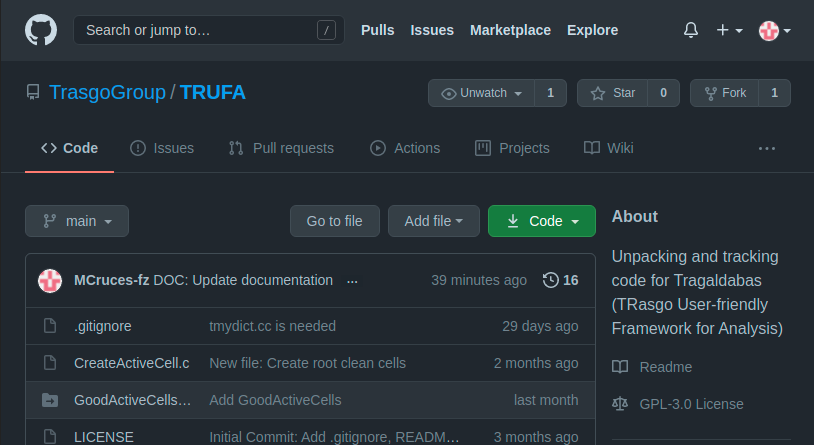
\includegraphics[width=\linewidth]{how_to_fork.png}}%
    \path[clip,rounded corners=10pt] (0,0) rectangle (\wd0,\ht0);
    \path (0.5\wd0,0.5\ht0) node[inner sep=0pt]{\usebox0};
    \end{tikzpicture}
    \caption{Example of main page of a repository.}
    \label{fig:Fork}
\end{figure}

